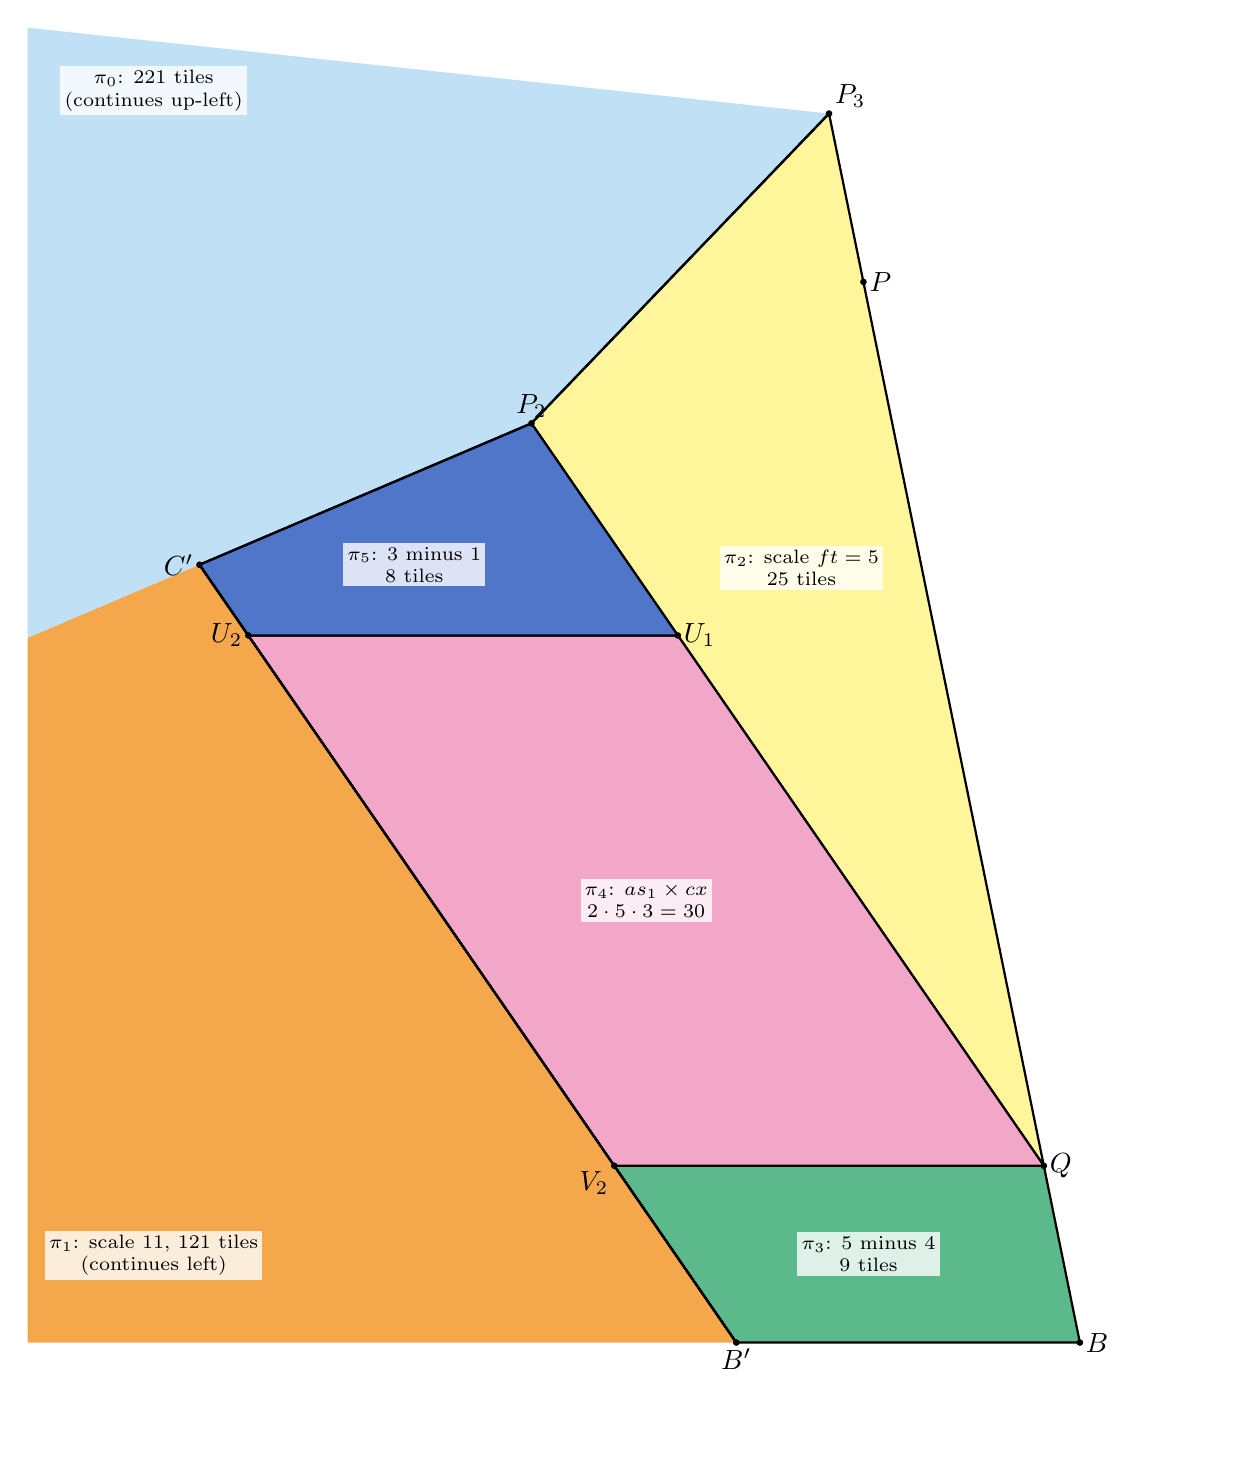
\begin{tikzpicture}[x=1cm,y=1cm,font=\footnotesize]
\definecolor{ef1}{HTML}{F4A74B}\definecolor{ef2}{HTML}{BFE0F5}\definecolor{ef3}{HTML}{5BB98C}\definecolor{ef4}{HTML}{FFF59A}\definecolor{ef5}{HTML}{4F76C9}\definecolor{ef7}{HTML}{F2A7C9}
\begin{scope}\clip (0,0) rectangle (15.000,17.790);
\fill[ef2] (10.177,16.699) -- (6.398,12.765) -- (0,10.039) -- (0,17.790) -- cycle;
\fill[ef1] (8.999,1.091) -- (2.182,10.969) -- (0,10.039) -- (0,1.091) -- cycle;
\fill[ef4,draw=black,line width=0.8pt] (10.177,16.699) -- (6.398,12.765) -- (12.905,3.336) -- cycle;
\fill[ef3,draw=black,line width=0.8pt] (13.363,1.091) -- (12.905,3.336) -- (7.450,3.336) -- (8.999,1.091) -- cycle;
\fill[ef7,draw=black,line width=0.8pt] (12.905,3.336) -- (8.257,10.071) -- (2.802,10.071) -- (7.450,3.336) -- cycle;
\fill[ef5,draw=black,line width=0.8pt] (8.257,10.071) -- (6.398,12.765) -- (2.182,10.969) -- (2.802,10.071) -- cycle;
\draw[line width=0.8pt] (10.177,16.699) -- (6.398,12.765); \draw[line width=0.8pt] (8.999,1.091) -- (2.182,10.969);
\draw[line width=0.8pt] (6.398,12.765) -- (2.182,10.969) -- (8.999,1.091);
\end{scope}
\fill (10.177,16.699) circle (1.2pt); \node[above right,inner sep=2pt] at (10.177,16.699) {\normalsize$P_3$};
\fill (6.398,12.765) circle (1.2pt); \node[above,inner sep=2pt] at (6.398,12.765) {\normalsize$P_2$};
\fill (12.905,3.336) circle (1.2pt); \node[right,inner sep=2pt] at (12.905,3.336) {\normalsize$Q$};
\fill (13.363,1.091) circle (1.2pt); \node[right,inner sep=2pt] at (13.363,1.091) {\normalsize$B$};
\fill (8.999,1.091) circle (1.2pt); \node[below,inner sep=2pt] at (8.999,1.091) {\normalsize$B'$};
\fill (2.182,10.969) circle (1.2pt); \node[left,inner sep=2pt] at (2.182,10.969) {\normalsize$C'$};
\fill (7.450,3.336) circle (1.2pt); \node[below left,inner sep=2pt] at (7.450,3.336) {\normalsize$V_2$};
\fill (8.257,10.071) circle (1.2pt); \node[right,inner sep=2pt] at (8.257,10.071) {\normalsize$U_1$};
\fill (2.802,10.071) circle (1.2pt); \node[left,inner sep=2pt] at (2.802,10.071) {\normalsize$U_2$};
\fill (10.614,14.561) circle (1.2pt); \node[right,inner sep=2pt] at (10.614,14.561) {\normalsize$P$};
\node[align=center,fill=white,fill opacity=0.8,text opacity=1,inner sep=1.5pt,font=\scriptsize] at (9.827,10.933) {$\pi_2$: scale $ft=5$\\$25$ tiles};
\node[align=center,fill=white,fill opacity=0.8,text opacity=1,inner sep=1.5pt,font=\scriptsize] at (10.679,2.214) {$\pi_3$: $5$ minus $4$\\$9$ tiles};
\node[align=center,fill=white,fill opacity=0.8,text opacity=1,inner sep=1.5pt,font=\scriptsize] at (7.854,6.703) {$\pi_4$: $as_1\times cx$\\$2\cdot5\cdot3=30$};
\node[align=center,fill=white,fill opacity=0.8,text opacity=1,inner sep=1.5pt,font=\scriptsize] at (4.910,10.969) {$\pi_5$: $3$ minus $1$\\$8$ tiles};
\node[align=center,fill=white,fill opacity=0.8,text opacity=1,inner sep=1.5pt,font=\scriptsize] at (1.600,16.990) {$\pi_0$: $221$ tiles\\(continues up-left)};
\node[align=center,fill=white,fill opacity=0.8,text opacity=1,inner sep=1.5pt,font=\scriptsize] at (1.600,2.200) {$\pi_1$: scale $11$, $121$ tiles\\(continues left)};
\end{tikzpicture}